\subsection{What the Historical Learned Study Establishes}
An earlier, separately frozen 126-condition comparison used the original 21-context trained models, including path counts up to 16 and SNRs down to $-10$~dB. On its 4,032 primary worlds, the 188-parameter controller improved equal-cell NMSE by 1.835~dB over global filtering and 1.967~dB over a matched recurrent adaptation, with adjusted intervals $[1.805,1.871]$ and $[1.932,2.006]$~dB. A per-block rank-selected OptShrink adaptation was 0.452~dB more accurate on that study's main score and substantially slower. These observations support the adaptive component under that training/test design; they are not results for the final hybrid or its current operating grid. The full historical comparisons, including contrary rankings under pooled error and alternative training, remain in the supplement.

\subsection{Fresh Accuracy, BER and Runtime}
\begin{table*}[!t]
\centering
\caption{Fresh 153-condition comparison. Lower values are better. Runtime is the slower of two independently timed windows, in milliseconds.}
\label{tab:reliability-main}
\small
\setlength{\tabcolsep}{4pt}
\begin{tabular}{lrrrrr}
\toprule
Method & \shortstack{Mean-cell\\NMSE (dB)} & \shortstack{Pooled linear\\NMSE} & BER (\%) & \shortstack{Full-grid\\p90 (ms)} & \shortstack{Weak-target\\p90 (ms)} \\
\midrule
Reliability receiver & -38.620 & 0.00897384 & 0.522496 & 7.254 & 7.031 \\
Prior selective EM & -38.113 & 0.00900482 & 0.522496 & 7.148 & 6.809 \\
Full repaired receiver & -37.858 & 0.00903694 & 0.522571 & 14.690 & 14.858 \\
Adaptive start + EM40 & -35.691 & 0.02637969 & 0.808204 & 9.040 & 8.704 \\
Global schedule + EM40 & -36.482 & 0.02658368 & 0.813718 & 7.103 & 6.745 \\
Classical start + EM40 & -32.005 & 0.02744311 & 0.809387 & 7.142 & 6.802 \\
Spectral EM100 & -30.562 & 0.02839215 & 0.828828 & 8.835 & 8.752 \\
Compact sparse/EM & -31.895 & 0.00868525 & 0.489159 & 9.516 & 8.756 \\
Algebraic start + EM20 & -36.534 & 0.02788204 & 0.835676 & 3.101 & 2.747 \\
\bottomrule
\end{tabular}
\par\vspace{2pt}
\begin{minipage}{0.98\textwidth}\footnotesize Neural rows average metrics from three separately evaluated fits, not ensembles. Mean-cell NMSE equally averages condition-level dB ratios of summed error to summed channel energy; pooled linear NMSE first pools all conditions within each fit and then averages the fit ratios. The weak target is RSR 5~dB and SNR $>30$~dB (24 conditions). The declared runtime target is 10.74~ms in both scopes and both windows; it is not a per-call deadline. Compact sparse/EM includes zero-penalty EM choices and remains best in pooled-linear NMSE and aggregate BER.\end{minipage}
\end{table*}

Table~\ref{tab:reliability-main} is the final, fresh matched comparison. The new receiver improves equal-cell mean NMSE by 0.507~dB over the prior hybrid, with adjusted interval $[0.338,0.652]$~dB, and by 0.762~dB over the full repair, with interval $[0.231,0.878]$~dB. The prior-relative fit-specific gains are 0.497, 0.504 and 0.521~dB. Gains over the full repair vary more, at 0.361, 0.114 and 1.810~dB; averaging fits does not remove this dependence on the trained weights.

Observed aggregate BER is identical for the new and prior hybrids: 0.522496\%. The full repair has 17 additional errors across the three fits, all in one fit, but the adjusted interval for BER improvement includes zero. We therefore claim no established BER improvement over either primary comparator. Compact sparse/EM is better in aggregate BER (0.489159\%) and pooled linear NMSE (0.008685 versus 0.008974). It also has smaller pooled error-tail summaries. The new receiver's best equal-cell mean dB score does not imply dominance under every error aggregation or in communication reliability.

\begin{figure*}[!t]
\centering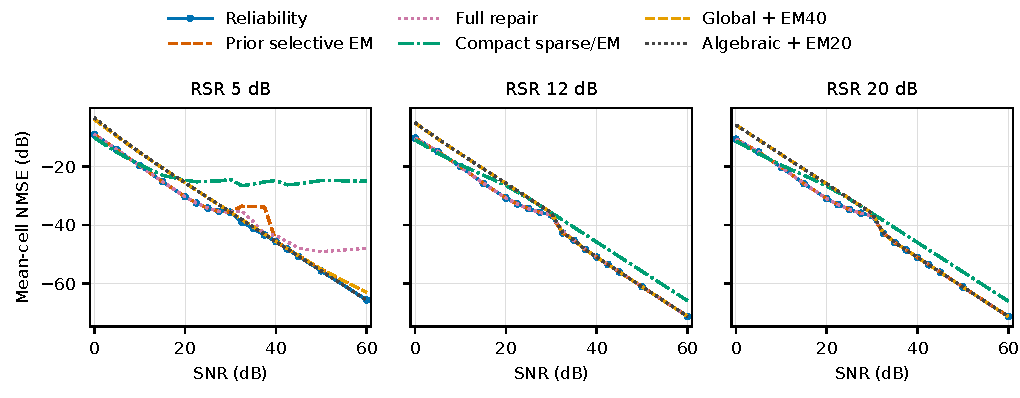
\includegraphics[width=\textwidth]{reliability_nmse.pdf}
\caption{Fresh final comparison. Each point averages the three path-regime cell NMSE scores; trained families additionally average three fit scores, not channel predictions. Curves are descriptive. All methods share observations. The algebraic-only and fixed-schedule controls show that classical recovery and a fixed trained schedule are strong at high SNR.}
\label{fig:reliability-nmse}
\end{figure*}
\begin{figure*}[!t]
\centering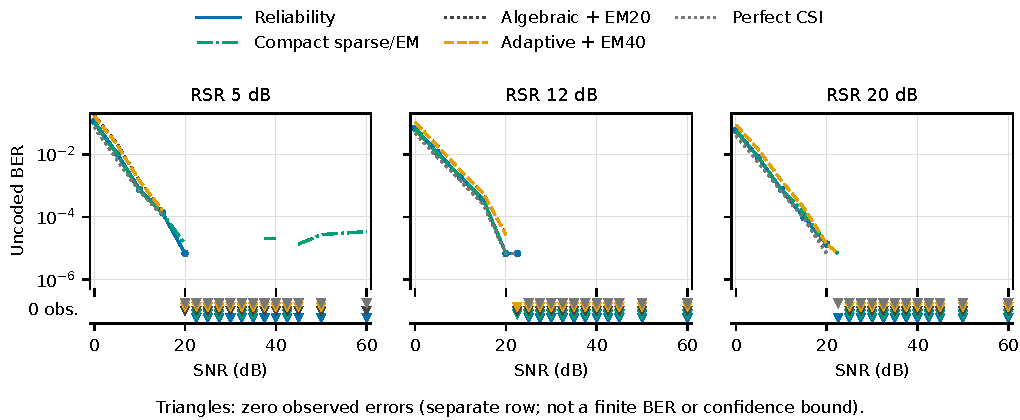
\includegraphics[width=\textwidth]{reliability_ber.pdf}
\caption{Estimate-then-detect BER on the same fresh observations and joint Rician detector. Points average path-regime rates, with equal case/bit counts. Zero-error observations appear in a separately labelled display row; they are not numerical upper bounds or evidence of equivalence. The perfect-CSI curve uses unavailable channel truth only as a detector diagnostic.}
\label{fig:reliability-ber}
\end{figure*}

\subsection{Where the New Check Helps and Where It Does Not}
\begin{table*}[!t]
\centering
\caption{Descriptive operating-range results on the same fresh bank.}
\label{tab:reliability-regions}
\small
\setlength{\tabcolsep}{4pt}
\begin{tabular}{llrrrrr}
\toprule
Region & Metric & Reliability & \shortstack{Prior selective\\EM} & Full repair & Sparse/EM & Algebraic20 \\
\midrule
Ordinary (45) & dB & -20.242 & -20.242 & -20.242 & -18.964 & -15.470 \\
 & BER (\%) & 1.776440 & 1.776440 & 1.776440 & 1.662191 & 2.841254 \\
Weak target (24) & dB & -48.644 & -45.411 & -43.893 & -25.607 & -48.457 \\
 & BER (\%) & 0.000000 & 0.000000 & 0.000480 & 0.001441 & 0.000000 \\
High SNR (45) & dB & -56.744 & -56.512 & -54.638 & -44.052 & -56.754 \\
 & BER (\%) & 0.000000 & 0.000000 & 0.000196 & 0.000633 & 0.000000 \\
\bottomrule
\end{tabular}
\par\vspace{2pt}
\begin{minipage}{0.98\textwidth}\footnotesize Ordinary: SNR $\leq20$~dB, all references. Weak target: RSR 5~dB and SNR $>30$~dB. High SNR: SNR $\geq40$~dB, all references. These scopes overlap and are not the multiplicity-adjusted primary comparisons. A displayed zero BER means no observed bit errors; it is neither a zero-error guarantee nor evidence of population equivalence. The first three methods are bitwise identical in the ordinary region.\end{minipage}
\end{table*}

The targeted region is reference 5~dB and SNR above 30~dB: 24 conditions. Here the receiver achieves $-48.644$~dB, improving on the prior by 3.232~dB, with descriptive interval $[2.249,3.966]$~dB, and on the full repair by 4.750~dB, with interval $[1.836,5.326]$~dB. Its pooled linear NMSE is $3.879\times10^{-5}$, versus $2.367\times10^{-4}$ for the prior. The fallback triggers on approximately 26.7--27.0\% of target cases across fits; every triggered fallback is accepted on this test bank and none has an invalid design. Trigger and acceptance remain separate decisions in the algorithm.

Fifteen of 153 condition-mean NMSE scores improve over the prior, with the remainder tied and none worse. This is a statement about the sampled condition means, not every individual channel. Ordinary-SNR outputs and all conditions outside the new gate are identical to the prior. Both methods have zero observed target-region bit errors, so the large channel-error gain has no measured BER benefit there.

The receiver does not beat the full repair in every cell: 32 condition means are worse, eight with pointwise intervals excluding zero. The largest mean loss is 0.701~dB at two paths, reference 20~dB and SNR 32.5~dB, outside the new gate. Under strong references at SNR at least 40~dB, its mean score is $-58.555$~dB versus $-58.558$~dB for the full repair. These residual losses are retained, rather than removed by test-dependent threshold changes.

Standalone algebraic-plus-EM20 is particularly competitive in the target region ($-48.457$~dB) and is the fastest tabulated pipeline. Its whole-grid BER, 0.835676\%, is substantially worse than the hybrid's. This supports combining components over the declared grid, while showing that learning is not necessary for accurate high-SNR recovery. The compact sparse/EM BER advantage is concentrated in ordinary-SNR operation, which this repair preserves rather than improves.

\subsection{Processing Budget and Latency Variability}
The new receiver passes both required p90 tests in both windows. Whole-grid p90 is 4.282 and 7.254~ms; target-region p90 is 4.162 and 7.031~ms. The fallback-triggered branch has p90 3.501 and 5.918~ms. Its conditional mix of operating points differs from that of untriggered calls, so these numbers do not imply that adding a fallback reduces cost. Every receiver reference/SNR-bin p90 also remains below 10.74~ms in the measured samples.

The slower second window affects the baselines as well. We retain both runs and report the worse p90; the full repair passes in the first window but fails in the second, at 14.690~ms overall and 14.858~ms in the target region. The final receiver has maximum measured times of 5.225 and 22.276~ms. One of its 1,377 calls in the second window exceeds 10.74~ms; its fallback gate was false. We do not assign a cause from these measurements. Thus the receiver meets the percentile target, not a hard per-call deadline.

\subsection{Negative Evidence and Scope}
The development record includes pilot-matched retraining, high-SNR bypass, weak-reference transition corrections, a filter-continuation repair around 40~dB, native-kernel runtime reduction and matched-start comparisons. These motivated the frozen final design. Earlier winners, failed confirmation tests and test-driven exploratory repairs are archived as development evidence, not independent confirmation of every component. No final-test outcome changes the selected rule.

Historical nearly noiseless tests exposed a large bias from nonvanishing learned filtering, even when initialized at the true channel. Historical variance and reference-phase perturbations also caused degradation. The final receiver has not been validated under those mismatches merely because its matched-model test is better. Known reference phase and variance remain required; constant reference-phase error can be absorbed by channel rotation and is not identified by a fitting-likelihood check. The current algebraic validity rule rejects constant-modulus fitting pilots. Array geometry, user counts other than three, hardware readout, nonlinear atomic dynamics and practical coded links require separate tests of the final pipeline.
